\documentclass{standalone}
\usepackage{amsmath, amsfonts, amsthm}
\usepackage[dvipsnames]{xcolor}
\usepackage{siunitx}
\usepackage{graphicx}
\usepackage{tikz}
\usepackage{circuitikz}
\usetikzlibrary{patterns}
\usepackage{scalerel}
\usepackage{pict2e}
\usepackage{tkz-euclide}
\usetikzlibrary{calc}
\usetikzlibrary{arrows.meta}
\usetikzlibrary{shadows}
\usetikzlibrary{external}
\usetikzlibrary{decorations.pathmorphing}
\usetikzlibrary{shapes.geometric}
\usetikzlibrary{arrows,shapes.gates.logic.US,shapes.gates.logic.IEC,calc}
\usepackage{pgfplots}
\pgfplotsset{compat=newest}
\usepgfplotslibrary{statistics}
\usepgfplotslibrary{fillbetween}

\begin{document}
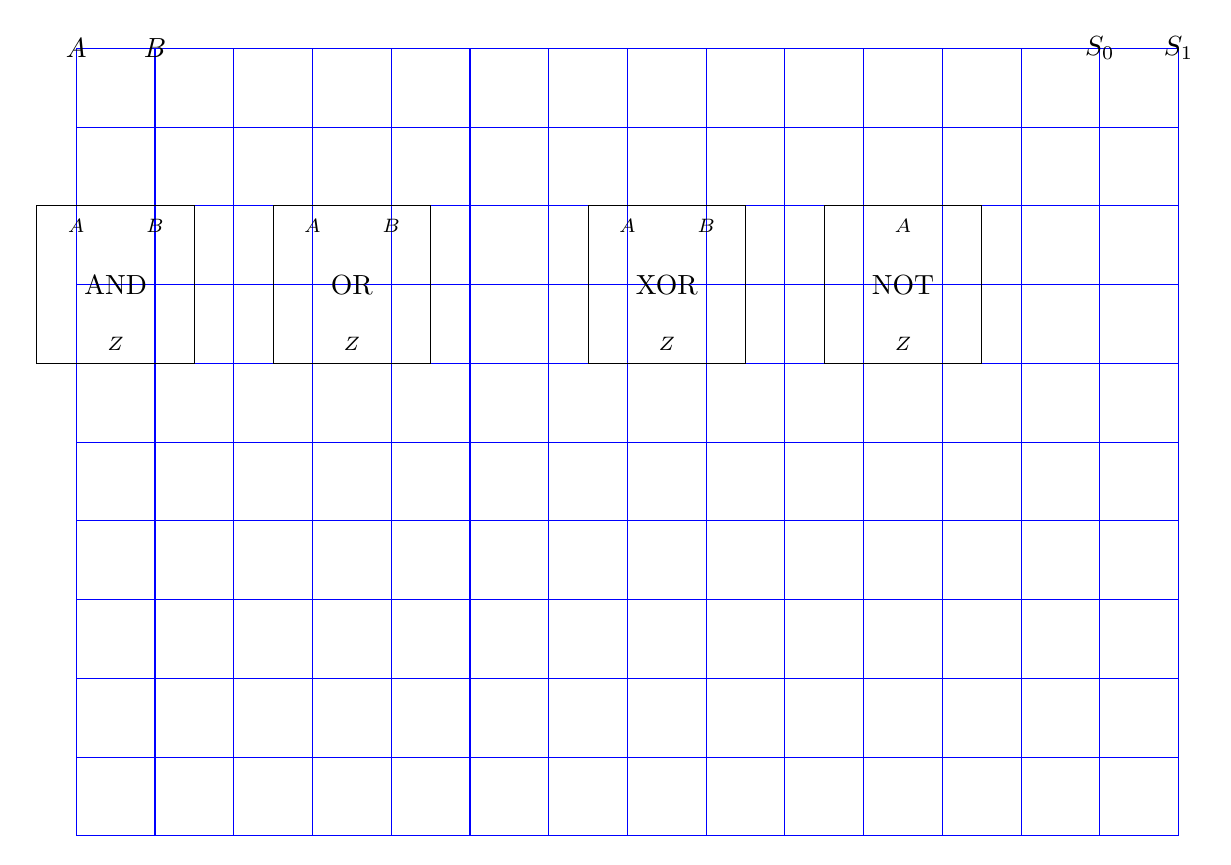
\begin{tikzpicture}
	%\draw [help lines, step=0.1, gray] (0,0) grid (10, -10);
	\draw [help lines, blue] (0,0) grid (14, -10);

	\node (A) at (0,0) {$A$};

	\node (B) [right of=A] {$B$};

	\node (S0) [right of=B, shift={(11, 0)}] {$S_0$};
	\node (S1) [right of=S0] {$S_1$};

	%And

	\node (AND) [below of=A, shift={(-.5, -1)}] { };
	\draw [black, thin] (AND) rectangle ++(2, -2);

	\node (AndA) [font=\scriptsize, right of=AND, shift={(-.5,-.25)}] {$A$};
	\node (AndB) [font=\scriptsize, right of=AndA] {$B$};

	\node (AndZ) [font=\scriptsize, below of=AndA, shift={(.5, -.5)}] {$Z$};

	\node (AndName) [above of=AndZ, shift={(0, -.25)}] {AND};

	%Or

	\node (OR) [right of=AND, shift={(2, 0)}] { };
	\draw [black, thin] (OR) rectangle ++(2, -2);

	\node (OrA) [font=\scriptsize, right of=OR, shift={(-.5,-.25)}] {$A$};
	\node (OrB) [font=\scriptsize, right of=OrA] {$B$};

	\node (OrZ) [font=\scriptsize, below of=OrA, shift={(.5, -.5)}] {$Z$};

	\node (OrName) [above of=OrZ, shift={(0, -.25)}] {OR};

	%Xor

	\node (XOR) [right of=OR, shift={(3, 0)}] { };
	\draw [black, thin] (XOR) rectangle ++(2, -2);

	\node (XorA) [font=\scriptsize, right of=XOR, shift={(-.5,-.25)}] {$A$};
	\node (XorB) [font=\scriptsize, right of=XorA] {$B$};

	\node (XorZ) [font=\scriptsize, below of=XorA, shift={(.5, -.5)}] {$Z$};

	\node (XorName) [above of=XorZ, shift={(0, -.25)}] {XOR};

	%NOT

	\node (NOT) [right of=XOR, shift={(2, 0)}] { };
	\draw [black, thin] (NOT) rectangle ++(2, -2);

	\node (NotA) [font=\scriptsize, right of=NOT, shift={(0,-.25)}] {$A$};

	\node (NotZ) [font=\scriptsize, below of=NotA, shift={(0, -.5)}] {$Z$};

	\node (NotName) [above of=NotZ, shift={(0, -.25)}] {NOT};

	\end{tikzpicture}
\end{document}
